\chapter{特殊结构网络}\label{cha:content4}
\section{特殊全连接网络}\label{section:complete_graph_cooperation}
{特殊全连接网络描述与求解}
在协作定位网络的问题模型下,给出下面三个简化条件:
\begin{enumerate}
\item 锚点测距方差$\sigma_i^2=\frac{1}{a}$
\item 未知节点彼此测距方差$\sigma^2_{ij}=\frac{1}{b}$
\item $\mathcal{E}=\{(i,j)|1\leq i <j\leq N\},N:=N_a,\angle\bm{u}_j=\frac{2\pi j}{n}$
\end{enumerate}
$I(\bm{p}_1,\dots,\bm{p}_N)$的最大特征值和最小特征值可由\textbf{瑞利商}求出,关于瑞利商有如下定理:
\begin{theorem}\label{theorem:rayleigh}
  设$\bm{A}$是一个对称正定的矩阵,设$\bm{v}_{\lambda}$为A的特征值$\lambda$对应的特征向量,则:
\begin{align*}
\begin{cases}
\lambda_{\text{max}}&=\max_{||\bm{x}||=1} \transpose{\bm{x}}\bm{A}\bm{x}\\
\bm{v}_{\lambda_{\text{max}}}&=\rgmax_{||\bm{x}||=1} \transpose{\bm{x}}\bm{A}\bm{x}
\end{cases}\quad
\begin{cases}
\lambda_{\text{min}}&=\min_{||\bm{x}||=1} \transpose{\bm{x}}\bm{A}\bm{x}\\
\bm{v}_{\lambda_{\text{min}}}&=\rgmin_{||\bm{x}||=1} \transpose{\bm{x}}\bm{A}\bm{x}
\end{cases}
\end{align*}
\end{theorem}

在条件(1),(2)成立的情况下,费舍尔信息矩阵$I(\bm{p}_1,\dots,\bm{p}_N)=a\bm{I}_{2N}+b\bm{J}$,其中
\[\bm{J}_{ij}=\begin{cases}
\sum_{k=1,k\neq i}^N \bm{u}_{ik}\bm{u}_{ik}^{\textrm{T}} &i=j\\
-\bm{u}_{ij}\bm{u}_{ij}^{\textrm{T}} &i\neq j,
\end{cases}
\]瑞利商为:
\begin{equation}
R(\bm{x})=b\sum_{i\leq j\leq N} (\bm{u}_{ij}^{\textrm{T}} (\bm{x}_i-\bm{x}_j))^2+a,\bm{x}_i\in \mathbb{R}^2
\end{equation}
容易看出,当$\bm{x}_i=\bm{x}_j$或$(\bm{x}_i-\bm{x}_j)$与$\bm{u}_{ij}$正交时,瑞利商$R(\bm{x})$取到最小值,
利用定理(\ref{theorem:rayleigh}),关于$I(\bm{p}_1,\dots,\bm{p}_N)$的特征值,我们有如下定理:
\begin{theorem}
如果简化条件1和2成立,那么$I(\bm{p}_1,\dots,\bm{p}_N)$的最大特征值是$a+Nb$,最小特征值是a;
如果三个简化条件均成立,那么$\mathbb{R}_{2N}=V_{a+Nb}\oplus V_a\oplus V_{a+Nb/2}$,且$dim(V_a)=3,dim(V_{a+Nb/2})=2N-4$
\end{theorem}
\begin{proof}
设$\mathring{p}_i$表示$\bm{p}_i$绕原点旋转$90^{\circ}$后的向量,$\bm{e}_1=(1,0),\bm{e}_2=(0,1)$,
容易看出
\[
V_a \supset\text{span}\{\{\bm{\mathring{p}_1},\bm{\mathring{p}_2},\dots,\bm{\mathring{p}} _N\},\{\bm{e}_1,\bm{e}_1,\dots,\bm{e}_1\},\{\bm{e}_2,\bm{e}_2,\dots,\bm{e}_2\}\}:=K_a
\]
下面证明$a+Nb$是$I(\bm{p}_1,\dots,\bm{p}_N)$的最大特征值,由Cauchy不等式:
\begin{align}\notag
R(\bm{y})&\leq b\sum_{i\leq j\leq N} ||\bm{u}_{ij}||^2||\bm{y}_i-\bm{y}_j||^2+a\\
&=b\sum_{i\leq j\leq N}||\bm{y}_i-\bm{y}_j||^2+a
\end{align}
取等条件是$\forall i,j\in \{1,2,...N\},i\neq j$,有$\bm{y}_i-\bm{y}_j$与$\bm{u}_{ij}$均平行,比如可以取
$\bm{y}_1-\bm{y}_j=k(\bm{p}_1-\bm{p}_j),j=2,...N$。
满足
$\bm{y}_i-\bm{y}_j=(\bm{y}_1-\bm{y}_j)-(\bm{y}_1-\bm{y}_i)
=k(\bm{p}_i-\bm{p}_j)\parallel \bm{u}_{ij}$
这时原来2N个自由度的y还剩下$\bm{y}_1$和k三个自由度,考虑条件极值
$f(\bm{y})=\sum_{i\leq j\leq N} ||\bm{y}_i-\bm{y}_j||^2,\text{s.t } ||\bm{y}||=1$
设矩阵T为:
\[
\bm{T}=\left(
\begin{array}{cccc}
(N-1)\bm{I}_2&-\bm{I}_2&\dots&-\bm{I}_2\\
-\bm{I}_2&(N-1)\bm{I}_2&\dots&-\bm{I}_2\\
\vdots & \vdots & \ddots & \vdots\\
-\bm{I}_2& -\bm{I}_2 & \dots & (N-1)\bm{I}_2
\end{array}
\right)
\]
$\bm{T}$可以写成$\bm{T}=N\bm{I}-\bm{e}\bm{e}^{\textrm{T}} $,其中$\bm{e}=(\bm{I}_2,\dots,\bm{I}_2)^{\textrm{T}} $。而$f(\bm{y})=\bm{y}^{\textrm{T}} \bm{T}\bm{y}=N-(\bm{e}^{\textrm{T}} \bm{y})^{\textrm{T}} (\bm{e}^{\textrm{T}} \bm{y})\leq N$取等条件是$\bm{e}^{\textrm{T}} \bm{y}=\bm{0}$,这个条件限制住了两个自由度,再加上$\bm{y}$模长为1的约束,前一次不等式取等剩下的三个自由度刚好够用,
所以$\bm{y}$按该方法可以唯一取到,其张成的子空间记为$K_b$。
具体求解可得:
$\bm{y}_1=\frac{k}{N}\sum_{j=2}^N (\bm{p}_1-\bm{p}_j)$
将$\bm{y}_i$的表达式代入$||\bm{y}||=1$中,可以解出唯一的$k^2=M$
其中
\[
M\sum_{i=1}^N||\sum_{j=1,j\neq i}^N(\bm{p}_1-\bm{p}_j)||^2=1
\]
  在条件(3)$\angle\bm{u}_j=\frac{2\pi j}{n}$的进一步假设下,设$\bm{x}\in (K_a\oplus K_b)^{\bot}$,
  下面证明$\bm{x}$是矩阵$\bm{J}$的特征值为$\frac{N}{2}$对应的特征向量。
  由正交性条件,有:
\begin{align}\notag
\sum \bm{x}_i^{(k)}&=0,k=1,2\\
\sum \bm{x}_i \cdot \bm{u}_i&=\sum x_i^{(1)} \cos(\frac{2\pi j}{n})+x_i^{(2)} \sin(\frac{2\pi j}{n})=0
\label{eq:coupling1}\\
\sum \bm{x}_i \cdot \mathring{\bm{u}}_i &=\sum -x_i^{(1)} \sin(\frac{2\pi j}{n})+x_i^{(2)} \cos(\frac{2\pi j}{n}) =0\label{eq:coupling2}
\end{align}
下面考虑$\bm{K}\cdot \bm{x}$的第j行为:
\begin{equation}\label{eq:tt}
\left(\bm{K}\cdot \bm{x}\right)_{(\cdot,j)}=\sum_{k\neq j}^n \frac{(\bm{u}_j-\bm{u}_k)^{\textrm{T}} (\bm{x}_j-\bm{x}_k)}{||\bm{u}_j-\bm{u}_k||^2}(\bm{u}_j-\bm{u}_k)
\end{equation}
我们要证明上面的式子等于$\frac{N}{2}\bm{x}_j$,为此,首先化简$\frac{(\bm{u}_j-\bm{u}_k)}{||\bm{u}_j-\bm{u}_k||}$
可以推出上式等于:
\begin{equation}
\frac{(\bm{u}_j-\bm{u}_k)}{||\bm{u}_j-\bm{u}_k||}=\text{sgn}(j-k)\binom{-\sin\frac{\pi(j+k)}{n}}{\cos\frac{\pi(j+k)}{n}}
\end{equation}
上面的式子中符号函数$\text{sgn}(j-k)$因为在式(\ref{eq:tt})中出现2次,所以相乘恒为1,它与求和指标k无关,可以作为公因子提取出来。
所以证明\[
\sum_{k\neq j}^n \frac{(\bm{u}_j-\bm{u}_k)^{\textrm{T}} (\bm{x}_j-\bm{x}_k)}{||\bm{u}_j-\bm{u}_k||^2}(\bm{u}_j-\bm{u}_k)=\frac{N}{2}\bm{x}_j
\]
化简为分别证明:
\begin{align*}
(*)\sum ((-\sin\frac{(j+k)\pi}{n},\cos\frac{(j+k)\pi}{n})\binom{x_j^{(1)}-x_k^{(1)}}{x_j^{(2)}-x_k^{(2)}})
\cos\frac{(j+k)\pi}{n}&=\frac{N}{2}x_j^{(2)}\\
(**)\sum ((-\sin\frac{(j+k)\pi}{n},\cos\frac{(j+k)\pi}{n})\binom{x_j^{(1)}-x_k^{(1)}}{x_j^{(2)}-x_k^{(2)}})
(-\sin\frac{(j+k)\pi}{n})&=\frac{N}{2}x_j^{(1)}
\end{align*}
(*)式等价于证明:
\[
\sum (-\sin\frac{(j+k)2\pi}{n},1+\cos\frac{(j+k)2\pi}{n})\binom{x_j^{(1)}-x_k^{(1)}}{x_j^{(2)}-x_k^{(2)}}=Nx_j^{(2)}
\]
在(\ref{eq:coupling1}),(\ref{eq:coupling2})式中,分别将(\ref{eq:coupling1})乘以$\sin(\frac{2\pi k}{n})$与(\ref{eq:coupling2})乘以$\cos(\frac{2\pi k}{n})$相减得:
\begin{equation}
\sum x_i^{(1)}\sin\frac{(j+k)2\pi}{n}-x_i^{(2)}\cos\frac{(j+k)2\pi}{n}=0
\end{equation}
利用上面这个等式即可证(*)式。
在(\ref{eq:coupling1}),(\ref{eq:coupling2})式中,分别将(\ref{eq:coupling1})乘以$\cos(\frac{2\pi k}{n})$与(\ref{eq:coupling2})乘以$\sin(\frac{2\pi k}{n})$相加得:
\begin{equation}
\sum x_i^{(1)}\cos\frac{(j+k)2\pi}{n}+x_i^{(2)}\sin\frac{(j+k)2\pi}{n}=0
\end{equation}
利用上面这个等式同理可证明(**)式。
\end{proof}
\begin{remark}
~\\
\begin{itemize}
  \item 当场景中各待测节点相距较近,而锚点离各待测节点较远时,\ref{section:circle_general}小节说明了各向同性是锚点最优部署的形态,如果考虑锚点相对于各待测节点的分布范围是最优部署的,那么上面对锚点部署使得其贡献的信息量为$a\bm{I}$的假设成立,在之后的讨论中,我们均持此假设。
  \item 假设3是说各待测节点分布在一个圆上,因为各待测节点相距较近,在圆周半径不是很小的情况下,可以近似认为各节点相互测距方差均相等,即假设2成立。
  \item 通过对特征值的倒数和取平均,每个节点的误差下界的量级是$\frac{4}{bN}$,\ref{section:circle_general}小节最优部署下非协作情形每个节点的误差下界的量级是$\frac{2}{aN}$,相比之下可以看出在a=b的情况下增加2个协作节点才有一个锚点的效果。
\end{itemize}

\end{remark}
\section{线型网络}\label{section:linear_network}
在动态协作定位网络的问题模型下,得到的费舍尔信息矩阵是三对角矩阵,在时间段[0,T]内,为研究减小时间间隔对定位性能的提高,我们需要对原来的模型作出如下的简化:
\begin{itemize}
\item 锚点测距方差$\sigma_i^2=\frac{1}{a}$
\item 未知节点彼此测距方差$\sigma^2_{ij}=\frac{1}{b}$
\end{itemize}
那么费舍尔信息矩阵式(\ref{eq:time_cooperation_matrix})可化简为
\begin{equation}\label{eq:Pab}
I(\bm{P})=a\bm{I}+b\bm{J}
\end{equation}
其中\[
J=\left(
\begin{array}{ccccc}
\bm{u}_{12}\bm{u}_{12}^{\textrm{T}} &-\bm{u}_{12}\bm{u}_{12}^{\textrm{T}} &\bm{0}&\dots&\bm{0}\\
&&&&\\
-\bm{u}_{12}\bm{u}_{12}^{\textrm{T}} &\bm{u}_{12}\bm{u}_{12}^{\textrm{T}} +\bm{u}_{23}\bm{u}_{23}^{\textrm{T}} &-\bm{u}_{23}\bm{u}_{23}^{\textrm{T}} &\dots&0\\
&&&&\\
\vdots &\vdots&\ddots &\vdots&\vdots\\
\bm{0}&\dots&\bm{0}&-\bm{u}_{N-1,N}\bm{u}_{N-1,N}^{\textrm{T}} &\bm{u}_{N-1,N}\bm{u}_{N-1,N}^{\textrm{T}} \\
\end{array}
\right)
\]
其中$K_1=\text{diag}\{1,0\}$,$Q=\text{diag}\{R_{\theta},...R_{\theta}\}$,$R_{\theta}$为二维旋转矩阵
求$\lim_{N\to \infty}\frac{\Tr(J^{-1})}{N}$


直接求解该问题需要如下两个引理:
\begin{lemma}\label{lemma:change}
设L是$m\times n$的矩阵,$a,\epsilon > 0$则
\begin{equation}
|a\bm{I}_m+\epsilon \bm{L}\bm{L}^{\textrm{T}} |=a^m|\bm{I}_n+\frac{\epsilon}{a} \bm{L}^{\textrm{T}} \bm{L}|
\end{equation}
\end{lemma}
\begin{proof}
不妨设$a=\epsilon=1$,
考虑到
\[
\left(\begin{array}{cc}
\bm{I}_n+\bm{L}^{\textrm{T}} \bm{L}&\bm{0}\\
\bm{L}&\bm{I}_m\\
\end{array}\right)\sim\left(\begin{array}{cc}
\bm{I}_n&-\bm{L}^{\textrm{T}} \\
\bm{L}&\bm{I}_m\\
\end{array}\right)\sim\left(\begin{array}{cc}
\bm{I}_n&-\bm{L}^{\textrm{T}} \\
0&\bm{I}_m+\bm{L}\bm{L}^{\textrm{T}} \\
\end{array}\right)
\]
其中$\sim$表示矩阵相抵,两边取行列式即得$|\bm{I}_m+\bm{L}\bm{L}^{\textrm{T}} |=|\bm{I}_n+\bm{L}^{\textrm{T}} \bm{L}|$,证毕。
\end{proof}


\begin{lemma}\label{lemma:special}
$\bm{S}$是一个n-1维的方阵,\[
\bm{S}=\left(
\begin{array}{cccc}
0&1&\dots&0\\
1&0&\dots&0\\
\vdots&\vdots&\ddots&\vdots\\
0&\dots&1&0\\
\end{array}\right)
\]则$\bm{S}$的n-1个特征值为:
$\lambda_j=2\cos(\frac{\pi j}{n}),j=1,2,...,n-1$
\end{lemma}
\begin{proof}
首先可以用数学归纳法证明S的特征多项式有递推公式:\[
P_n(\lambda)=\lambda P_{n-1}(\lambda)-P_{n-2}(\lambda)
\]
$P_n(\lambda)$对应n维的S。
其次证明
\[
U_n(\lambda)=\frac{1}{\sqrt{1-(\frac{\lambda}{2})^2}}\sin((n+1)\arccos(\frac{\lambda}{2}))
\]
适合上面的递推关系式。
最后证明$U_n(\lambda)$是关于$\lambda$的多项式,而这只需要证明$U_1(\lambda),U_2(\lambda)$是多项式即可。
\end{proof}

$\bm{I}(\bm{p}_1,\dots,\bm{p}_N)$的特征多项式为\[
p(\lambda)=|(\lambda-a)\bm{I}-b\bm{L}\bm{L}^{\textrm{T}} |
\]
其中L是2N乘以N的矩阵:
\[
L=\left(
\begin{array}{ccccc}
\bm{u}_1&0&\dots&&0\\
-\bm{u}_1&\bm{u}_2&0&\dots&0\\
0&-\bm{u}_2&\bm{u}_3&\dots&0\\
\vdots &\vdots&&\ddots &\vdots\\
0&\dots&0&-\bm{u}_{N-1}&0\\
\end{array}
\right)
\]
为获得该多项式的全部零点,我们进一步设$u_i=(1,0)^{\textrm{T}} $,即目标节点作直线运动,后面可以看到直线运动对应着误差最小的情形。
根据引理(\ref{lemma:change}),
\[
|(\lambda-a)\bm{I}-bLL^{\textrm{T}} |=(\lambda-a)^{2N}|\bm{I}_n-\frac{b}{\lambda-a}L^{\textrm{T}} L|
\]
$L^{\textrm{T}} L$是N阶方阵:
\[
L^{\textrm{T}} L=\left(
\begin{array}{ccccc}
2&-1&\dots&&0\\
-1&2&-1&\dots&0\\
0&-1&2&\dots&0\\
\vdots &\vdots&&\ddots &\vdots\\
0&\dots&&0&0\\
\end{array}
\right)
\]
设$\bm{K}_{N-1}$为$L^{\textrm{T}} L$第N-1阶主子式,则
\[
|(\lambda-a)\bm{I}-bLL^{\textrm{T}} |=(\lambda-a)^{N+1}|(\lambda-a)\bm{I}_{N-1}-b\bm{K}_{N-1}|
\]
设$n:=N$,则$\bm{K}_{n-1}=2\bm{I}_{n-1}-\bm{S}$,由引理(\ref{lemma:special})可求出$\bm{I}(\bm{p}_1,\dots,\bm{p}_N)$的全部特征值。
\[
f(n)=\frac{\Tr(J^{-1})}{n}==\frac{1}{n}\left(\frac{n+1}{a}+\sum_{j=1}^{n-1}\frac{1}{a+2b(1-\cos(\frac{\pi j}{n}))}\right)
\]
当$n\to \infty$,根据Riemann积分的定义:
\[
\lim_{n\rightarrow \infty}f(n)=\frac{1}{a}+\int_0^1 \frac{1}{a+2b(1-cos(\pi x))}dx
\]
化为复积分由留数定理可得\[
\lim_{n\rightarrow \infty}f(n)=\frac{1}{a}+\frac{1}{\sqrt{a^2+4ab}}
\]

直接从定义求解上面的问题较繁琐,下面用\textbf{Schur补}(Schur Complement)求解该问题:
%EFIM的思路是说,如果我们只关心场景中单个移动节点的定位误差,则可以通过分块矩阵的思路对总体的FIM进行分解。

\begin{definition}
    设矩阵$I=\left(\begin{array}{cc}A&B\\C&D\end{array}\right)$,那么矩阵$I$关于D的Schur补定义为$
    I/\ D=A-BD^{-1}C$,若$I^{-1}$与I作同样的分块,则$(I/\ D)^{-1}$是$I^{-1}$左上角的分块矩阵。
\end{definition}
\begin{remark}
	在我们的应用场景中,矩阵$I$是费舍尔信息矩阵,可以证明$(I/\ D)$给出于参数空间$\Theta$的子空间的费舍尔信息矩阵,计算$\text{tr}(I^{-1})$可以分解为计算各个子空间的误差再求和,一般取子空间的大小为2维,对应着一个位置的XY坐标。$I/\ D$在我们的应用场景中也称为等效费舍尔信息矩阵(Equivalent Fisher Information Matrix)。
\end{remark}
{用Schur补求解节点平均定位误差}
我们将用连分式的数学方法分析问题,在此之前给出一些关于连分式的基本结论\cite{ContinuedFraction}:
\begin{definition}
  有限序列$t_1,t_2,\dots,t_r$满足$t_j\geq 1$对于$j\geq2$可以递推地定义有限连分式
  \[[t_1,t_2,\dots,t_r]:=t_1+\frac{1} {[t_2,\dots,t_r]}\]
\end{definition}
\begin{theorem}\label{thm:basic}
  设$p_j=t_j p_{j-1}+p_{j-2},q_j=t_j q_{j-1}+q_{j-2}$,$M_j=\left(\begin{matrix}p_j&p_{j-1}\\q_j&q_{j-1}\end{matrix}\right)$
  $p_0,p_1,q_0,q_1$由$M_0=I_2$给出,且$T_j=\left(\begin{matrix}t_j&1\\1&0\end{matrix}\right)$则有下面三个恒等式:
  \begin{enumerate}
    \item $M_j=M_{j-1}T_j$
    \item $\binom{p_j}{q_j}=(\prod_{i=1}^r T_i )\binom{1}{0}$
    \item $[t_1,t_2,\dots,t_r]=\frac{p_r}{q_r}$
  \end{enumerate}
\end{theorem}
\begin{theorem}\label{theorem:quadratic_cyclic}
若$\lim_{r\to \infty}[t_1,t_2,\dots,t_r]$存在,该极限是形如$\frac{a+b\sqrt{m}}{c}$的二次根式当且仅当序列$t_i$从某项开始是周期的,即$\exists c,rc,\,s.t.\, t_{i}=t_{i+r},\forall i\geq c$。
\end{theorem}
\begin{remark}
对于定理\ref{theorem:quadratic_cyclic},设$\left(\begin{matrix}a&b\\c&d\end{matrix}\right)=(\prod_{i=1}^{rc} T_{i+c})$,称$\left(\begin{matrix}a&b\\c&d\end{matrix}\right)$对应着分式线性变换K,如果$K(z)=\frac{az+b}{cz+d}$。
可以证明系数为实数的分式线性变换以函数复合作为群运算与行列式为1的2阶方阵以矩阵乘积作为群运算是同构的。
c之前的$t_i$对应着矩阵$T_i$的乘积矩阵看作分式线性变换F。可以进一步说明二次根式和T和F的有如下的关系:
\begin{enumerate}
  \item 首先求解$K$的不动点即解二次方程$x=\frac{ax+b}{cx+d}$得x
  \item $F(x)=\lim_{r\to \infty}[t_1,t_2,\dots,t_r]$,F(x)即为极限$\lim_{r\to \infty}[t_1,t_2,\dots,t_r]$
\end{enumerate}
一般二次方程有两个根,而有限连分式的极限值是唯一的,这时可根据极限值介于序列的前两个数之间剔除一个不合理的不动点。
\end{remark}
应用连分式的基本理论,我们对式\ref{eq:Pab}中$a\bm{I}+b\bm{J}$提取b,记$\lambda=\frac{a}{b}$
通过Schur补的公式可以推导出关于矩阵$(\lambda\bm{I}+\bm{J})$左上角的2乘2矩阵的Schur补一个特征值是$\lambda$,另一个特征值$T_1$可以用下面的递归方法得到
\begin{equation}\label{eq:recursive_efim}
\begin{split}
\underbrace{T_{i-1}-\lambda}_{M} & =\frac{1}{1+\frac{\sin^2\theta_i}{\lambda}+\frac{\cos^2\theta_i}{T_i}},2\leq i\leq N_a-1\\
T_{N_a-1} & = \lambda+\frac{1}{1+1/\lambda}
\end{split}
\end{equation}
其中$\theta_i=\angle (\bm{p}_{t_i}-\bm{p}_{t_{i-1}},\bm{p}_{t_i}-\bm{p}_{t_{i+1}})$。
%Ti should be described by symbol, not natural language.
具体推导过程详见附录[\ref{B_F_1}]

这个求解是针对目标节点的记时起点或终点而言的,如果针对其时间中点,则其可分别看成两段轨迹的起点和终点,
其费舍尔信息矩阵为:$\bm{I}_p=\lambda I+M_1\bm{u}\bm{u}^{\textrm{T}} +M_2\bm{v}\bm{v}^{\textrm{T}} $
其中$\bm{u},\bm{v}$是与目标位置$\bm{p}$直接相连的两个位置$\bm{p}_1,\bm{p}_2$与目标节点的方向向量。$M_1,M_2$满足递推公式(\ref{eq:recursive_efim}),
但具体角度参数可能不一样,假设$N_a$是奇数使得时间中点存在于待测位置中,于是每个M算到$\frac{N_a+1}{2}$
但如果我们考虑的是$N_a\to \infty$的情形,则不受终止位置的限制。
$\bm{I}_p$的两个特征值为可由式(\ref{eq:Lambda})得出:
\[
\lambda_{1,2}=\lambda+\frac{M_1+M_2\pm \sqrt{M_1^2+M_2^2+2M_1M_2\cos2\phi}}{2}
\]
$\phi$为夹角$\angle(\bm{p}_1-\bm{p},\bm{p}_2-\bm{p})$,注意到时间中点时两个特征值均比$\lambda$大。
我们先考虑所有$\bm{u}_i=(1,0)^{\textrm{T}} $的特殊情形,此时一个特征值为$\lambda$,另一个特征值写成连分式为:
\begin{equation}\label{eq:gcf_1}
\lambda+\frac{2}{[1,\lambda,1,\lambda,\dots]}=\lambda+\cfrac{2}{1+\cfrac{1}{\lambda+\cfrac{1}{1+\cfrac{1}{\lambda+\dots}}}}
\end{equation}
我们先求循环的部分的连分式的值K,然后代入$\lambda+2/K$中即可
K对应的迭代矩阵循环周期为2,
写成$\begin{pmatrix}1 & 1 \\1 & 0\end{pmatrix}\begin{pmatrix}\lambda & 1 \\1 & 0\end{pmatrix}$
解方程$x=\frac{(\lambda+1)x+1}{\lambda x+1}$并考虑到解$x>0$,得$K=\frac{\lambda+\sqrt{4\lambda+\lambda^2}}{2\lambda}$,
最后得时间中点所求的目标节点的误差下界为$\sqrt{\lambda^2+4\lambda}$。同理,将式\ref{eq:gcf_1}中分子2改为1求出对应于时间起点或终点
误差下界为
\begin{align}\notag\label{eq:starting_or_ending}
M^*:&=[\lambda,1,\lambda,1,\dots]\\
&=\frac{\lambda+\sqrt{4\lambda+\lambda^2}}{2}
\end{align}

从时间间隔起始位置误差下界的一般表达式可以看出:
\begin{enumerate}
  \item Schur补做特征值分解后,在一个方向上的信息量始终为$\lambda$,减小时间间隔也无法改善;
  \item 另一个方向上信息量随$N_a$增大而增大,但有一个上界,粗略的讲不可能超过$\lambda+1$
  \item 若某两次时间间隔夹角正交,则$\cos\theta_i=0$之后的所有位置均不能对时间间隔起始位置的定位有贡献。
\end{enumerate}
对于一般的情形,当时间间隔比较小时,有理由假设角度不会有大的突变,且若轨迹的切向量如果是连续变化的,那么时间间隔充分小,前后两次测量间
角度可认为不变,那么有理由认为之前求的$M^*$是对一般的曲线轨迹在$\Delta t\to 0$时成立。我们有下面的定理,证明可参考附录[\ref{B_F_6}]
\begin{theorem}\label{theorem:arbitrary_curve}
若平面轨迹曲线参数化形式为$t\in[0,1]\rightarrow \bm{p}(t)=(x(t),y(t))$,满足
\begin{itemize}
\item $\bm{p}(t_1)\neq \bm{p}(t_2),\forall t_1\neq t_2$
\item $\bm{p}'(t)$存在且连续
\end{itemize}
对[0,1]区间有分割$0=t_1<t_2<\dots<t_{N_a-1}<t_{N_a}=1$,
记$\Delta t=\max_{1\leq i\leq N_a-1}|t_{i+1}-t_i|$
则式(\ref{eq:recursive_efim})给出的$T_1(N_a)$满足:
\begin{equation}\label{eq:limiting_cf}
\lim_{\Delta t\to 0}T_1(N_a)=M^*
\end{equation}
\end{theorem}

下面我们对不同的轨迹做数值计算,结果如图\ref{figure:tend_to_limit}所示
\begin{figure}
  \centering
  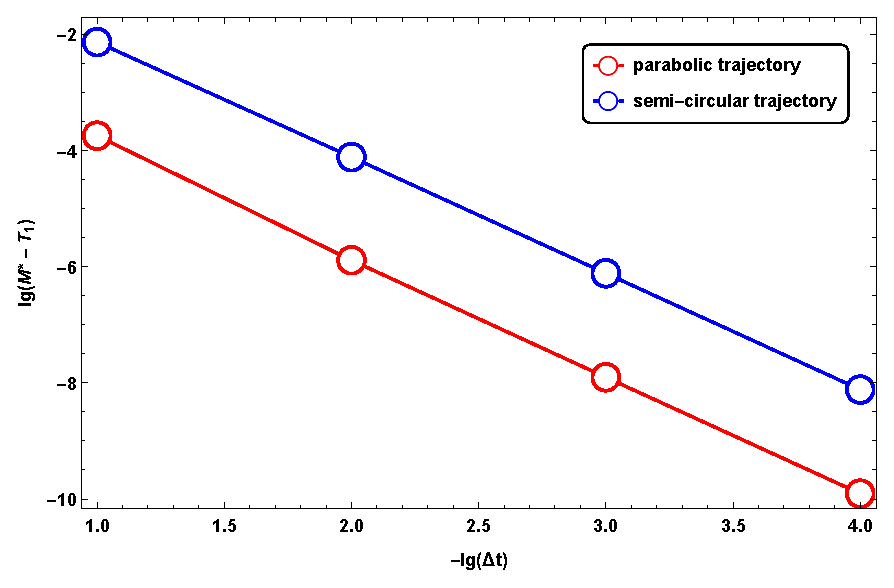
\includegraphics[width=400pt]{different_curve.eps}
  \caption{$\lambda=2$时不同曲线随采样点加密趋近极限值的情况;其中抛物轨迹对应的曲线是$(t,t^2)$,半圆轨迹是$(\cos(\pi t),\sin(\pi t))$}\label{figure:tend_to_limit}
\end{figure}
%圆弧仿真
由图\ref{figure:tend_to_limit}可见,
\begin{itemize}
  \item 随着$\Delta t$的减小,各种曲线均二次收敛于极限值,二次收敛的结果可以从log-log图的斜率是2印证,
而从定理\ref{theorem:arbitrary_curve}的证明过程的式(\ref{eq:quatratic_convergence})中出现$\Delta t$的平方可见证明过程的合理性。
  \item 对于不同的曲线,虽然收敛速度的量阶一致,但由于角度变化上有快有慢,所以体现在图中还是有高有低,平均来说,半圆弧在一个时间单位中角度变化了180度,而抛物线只有不到60度,角度变化越小相对更接近直线状态,因而收敛地更快些。
\end{itemize}
虽然$\sqrt{\lambda^2+4\lambda}$是一个最大的信息量,但下面的定理指出,较远的时间间隔的位置的贡献实际上是幂指数衰减的,证明见附录[\ref{B_F_2}]:
\begin{theorem}\label{theorem:exponential_decreasing}
若相邻时间间隔最大的角度变化量小于$\Delta \theta$,则由式(\ref{eq:recursive_efim})确定的数列$T_1(N_a)$(简记为$T_{N_a}$)的增量$\Delta_{+} T_{N_a}:=T_{N_a+1}-T_{N_a},\Delta_{+} T_{1}=\frac{\lambda}{\lambda+1}$,$N_a\geq 2$时满足:
\[
\frac{(\cos\Delta\theta)^{2(N_a-1)}}{(1+1/\lambda)^2(\lambda^2+2\lambda)(2+\lambda)^{2(N_a-2)}}\leq \Delta_{+} T_{N_a}\leq\frac{1}{(\lambda^2+2\lambda)(1+\lambda)^{2(N_a-2)}}
\]
\end{theorem}
\begin{remark}
由于费舍尔信息随链路是幂指数衰减,再对某一时刻的目标节点进行定位时,只需考虑前后几个时刻的位置即可,较远的时刻基本没有信息量,利用上只会增加计算上的开销而对定位性能不会有多大的提升。

为说明此结论,我们对式\ref{eq:recursive_efim}取不同的$\lambda$进行简单的数值计算,其中$\theta_i$按照~\ref{section:temporal_cooperative_localization}小节中$[0,2\pi]$均匀分布的假设求不同的$N_a$时$T_i$的性能平均,结果图~\ref{fig:continuous_fraction_exponential}所示:
\begin{figure}
  \centering
  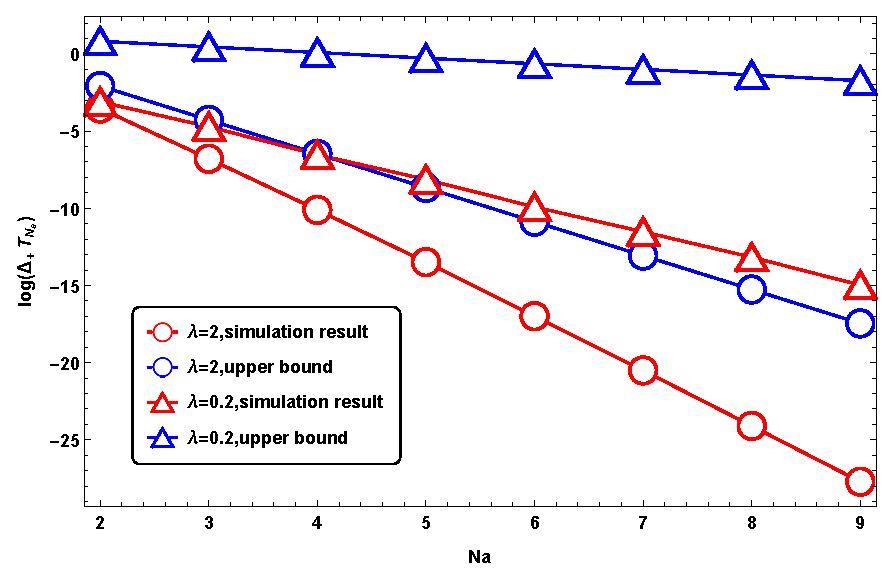
\includegraphics[width=400pt]{decreasing_exponential.eps}
  \caption{连分式指数收敛性图示}\label{fig:continuous_fraction_exponential}
\end{figure}
根据图~\ref{fig:continuous_fraction_exponential}可以看出:
\begin{itemize}
\item 通过蒙特卡罗仿真进一步验证了定理~\ref{theorem:exponential_decreasing}的正确性。
\item $\lambda=\frac{a}{b}$,表示锚点定位强度与目标节点协作强度之比,当$\lambda$较大即锚点定位更强时,图中协作信息量下降得更快,表明更远的协作链路所能提供的信息更少。
\item 实际随机模拟中的信息衰减速度要快于定理~\ref{theorem:exponential_decreasing}给出的上界,这主要是因为随机模拟中出现角度正交的情况时会阻断信息量从较远链路的传播。为了讨论信息衰减下界,我们取$\lambda=1$,并假设链路的夹角$\theta_i$服从零均值的正态分布,对于给定的$\Delta \theta$标准差$\sigma$满足$3\sigma=\Delta \theta$,由$3-\sigma$原则可近似认为角度变化不会超过$\Delta$,数值结果如图\ref{fig:continuous_fraction_exponential_lower_bound}所示
    \begin{figure}
      \centering
      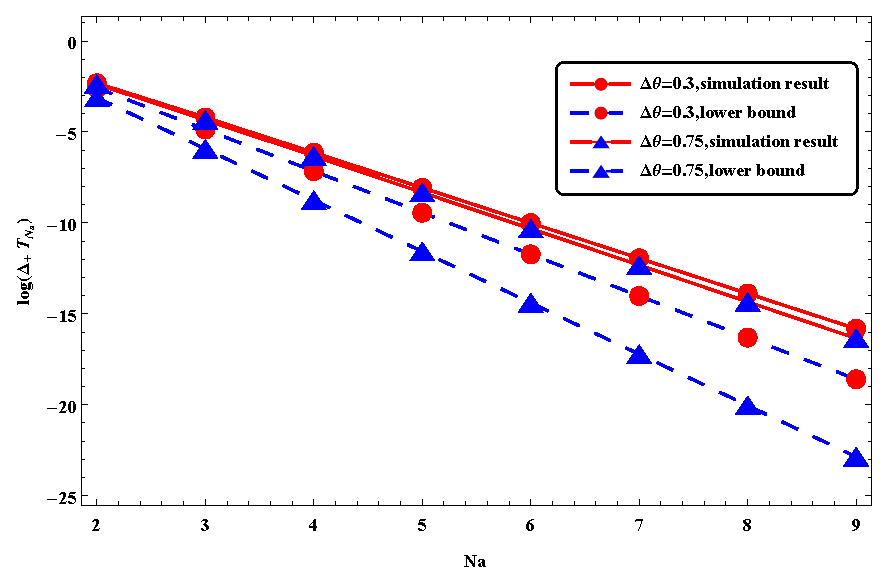
\includegraphics[width=400pt]{decreasing_exponential_lower_bound.eps}
      \caption{连分式指数衰减下界图示}\label{fig:continuous_fraction_exponential_lower_bound}
    \end{figure}

    分析图\ref{fig:continuous_fraction_exponential_lower_bound}可知,对于同等定位强度,如果目标节点角度变化得比较快,则信息衰减得也更快,多条链路后的位置将提供更少的信息量。
\end{itemize}
\end{remark}
\begin{remark}
在\ref{section:temporal_cooperative_localization}小节中,推导得出两个节点时间一次协作的模型问题可以转化为单节点的模形,但存在一个区别在于这里各时刻速度方向$\theta_i$是随机变量,因此求得的SPEB$\frac{1}{\lambda}+\frac{1}{T_1}$是关于$\theta_i$的随机变量,要对其求数学期望才能得到平均性能。

沿用式\ref{eq:recursive_efim}的假设,对诸$\theta_i$求平均后即得平均性能,由于是连分式的形式无法显式给出平均后的结果,但在后续仿真中我们将分别采用蒙特卡罗模拟的方法估计这个平均性能。

另外由于定理~\ref{theorem:exponential_decreasing}中的信息衰减上下界不含$\theta$,因此也是平均性能提升的衰减速率。如果针对两个节点时间协作的模型问题,则应
估计$\sum_{i=N_a}^{2N_a}\frac{1}{q^{2i}}$,结果还是$q^{2N_a}$量级,即$N_a$层后面的所有链路的增益与第$N_a$层的增益相当,即我们有如下推论,详见附录[\ref{B_F_5}]:
\end{remark}
\begin{corollary}[定理\ref{theorem:exponential_decreasing}的推论]\label{corollary:exponential_decreasing}
在定理\ref{theorem:exponential_decreasing}的的条件下,数列$\{T_{N_a}\}$收敛于$T_{\infty}$,收敛速度是指数收敛的,即\[
\exists q>1,C>0,s.t. |T_{N_a}-T_{\infty}|\leq\frac{C}{q^{N_a}}
\]
\end{corollary}
上面的推导过程具有一般性,下面我们不对未知节点测距方差作出相等的假设,则对$a\bm{I}+b\bm{J}$提取a,并设$\lambda_{ij}=\frac{b}{a\sigma_{ij}^2}$于是我们只需考虑$\bm{I}+\bm{J}$,其中
\[\scriptsize{
J=\left(
\begin{array}{ccccc}
\lambda_{12}\bm{u}_{12}\bm{u}_{12}^{\textrm{T}} &-\lambda_{12}\bm{u}_{12}\bm{u}_{12}^{\textrm{T}} &\bm{0}&\dots&\bm{0}\\
&&&&\\
-\lambda_{12}\bm{u}_{12}\bm{u}_{12}^{\textrm{T}} &\lambda_{12}\bm{u}_{12}\bm{u}_{12}^{\textrm{T}} +&-\lambda_{23}\bm{u}_{23}\bm{u}_{23}^{\textrm{T}} &\dots&0\\
&\lambda_{23}\bm{u}_{23}\bm{u}_{23}^{\textrm{T}} &&&\\
\vdots &\vdots&\ddots &\vdots&\vdots\\
\bm{0}&\dots&\bm{0}&-\lambda_{N-1,N}\bm{u}_{N-1,N}\bm{u}_{N-1,N}^{\textrm{T}} &\lambda_{N-1,N}\bm{u}_{N-1,N}\bm{u}_{N-1,N}^{\textrm{T}} \\
\end{array}
\right)}
\]
类似式~(\ref{eq:recursive_efim}),
我们可以导出目标节点Schur补一个特征值为1,另一个特征值$T_1$满足下面的递推关系式:
\begin{equation}\label{eq:recursive_efim_second}
  T_i=\frac{1}{\lambda_{i,i+1}^{-1}+\sin^2\theta_i+\frac{\cos^2\theta_i}{T_{i+1}}}
\end{equation}
其基本形式和(\ref{eq:recursive_efim})相同,计算算到$T_{N_a}=1$,
具体推导过程可参考[\ref{B_F_3}]

并且可以证明,减小诸$\theta$可以提高$T_1$即增大信息量,因此在线性网络中,当目标节点作直线运动时,确定其各个时刻的位置获得的信息量最大,因而精度最高。
\section{正方形网络与正六边形网络}\label{section:square_and_hexagon_network}
在协作定位网络的问题模型下,我们利用Schur补的数学工具,考虑大规模空间协作两种特殊的情形:
正方形网络和正六边形网络。正六边形网络的每个内部节点周围有3个节点与之协作,且该内部节点位于周围三个节点构成的正三角形的重心上。
为研究正六边形网络对定位性能的影响,我们考虑以一个节点$\bm{p}$为网络中心,我们称网络中某节点$\bm{p}_n$位于第n层链路上如果$\bm{p}_n$到$\bm{p}$的最短路径为n,图\ref{HexagonNetwork}就是一个只考虑前两层链路的正六边形网络。
\begin{figure}[h]
  \centering
  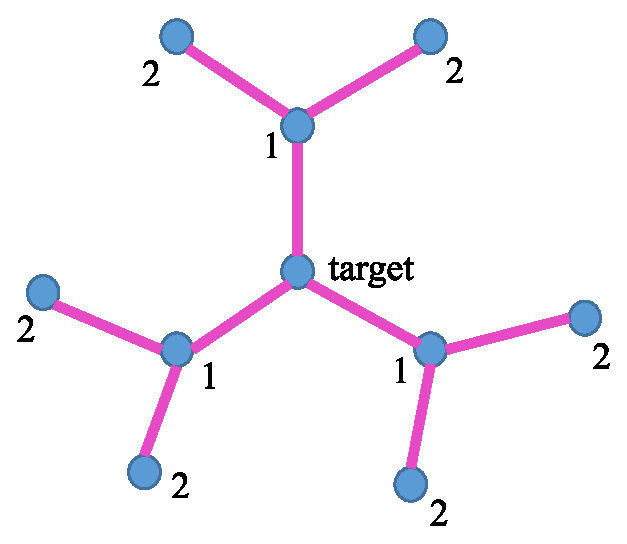
\includegraphics[width=250pt]{massive_spatial.eps}
  \caption{只考虑前两层链路的正六边形网络}\label{HexagonNetwork}
\end{figure}

正方形网络的描述同正六边形网络,如果以目标节点作为坐标原点,含其他未知位置的节点的两条直线作为坐标轴建立平面直角坐标系,
根据前面的正交性的结论,非坐标轴上的点不会对目标节点提供定位信息,而两条坐标轴提供的信息又彼此独立,因此其定位信息量是2个完全相同的部分相加,
每部分由式(\ref{eq:gcf_1})描述,在网络规模很大时近似于极限值$\sqrt{\lambda^2+4\lambda}$。

该结论可以推广至一般矩形网络,且各节点相互测距的方差$\sigma^2_{i,j}$不相等,由式(\ref{eq:recursive_efim_second})可以看出正交性的结论仍然成立,因此非坐标轴上的点不会对目标节点提供定位信息,在实际定位系统的设计中,非坐标轴上的点的信息无需传到目标节点或中央处理器进行解算。

下面我们给出大规模正六边形网络目标节点定位误差界的解析表达式,首先需要下面的引理,推导过程见附录[\ref{B_F_4}]
\begin{lemma}\label{lemma:hexagon}
  设$u$是模长为1的平面向量,那么有:
\begin{equation}\label{eq:equiv}
  u^{\textrm{T}} ((\lambda+\frac{3}{2})I_2-\frac{1}{\lambda+\frac{3}{2}}(\frac{3}{2}I_2-uu^{\textrm{T}} ))^{-1}u
  =((\lambda+\frac{3}{2})-\frac{1/2}{\lambda+\frac{3}{2}})^{-1}
\end{equation}
\end{lemma}
  上面的引理能够把连分式中与$u$相关的项化为与$u$无关的项,由此推出度为3的协作网络中心节点SPEB满足:
  \[
\frac{1}{\text{SPEB}}=\lambda+\frac{3}{2}-\cfrac{3/2}{\lambda+\frac{3}{2}-\cfrac{1/2}{\lambda+3/2-\dots}}
  \]
  注意到除了第一层的协作外,后面每层协作由于前一层的削弱系数由3/2变为1/2.
  用同样的方法可求出极限值为:
  \[
  \lambda+\frac{3}{2}-\cfrac{3/2}{\lambda+\frac{3}{2}-\cfrac{1/2}{\lambda+3/2-\dots}}=\sqrt{\lambda^2+3\lambda+\frac{1}{4}}-\frac{1}{\lambda+\frac{3}{2}+\sqrt{\lambda^2+3\lambda+\frac{1}{4}}}
  \]
  取倒数即为某方向的误差下界,由于网络的各向同性,x方向和y方向的误差下界都是这个数。
该误差下界总是比正方形网格x或y方向的误差大。

\section{本章小节}\label{section:conclusion4}
  % Keep the summary *very short*.
   本章中的主要结果除引用连分式的基本结论外,大都是原创性的,而且不乏有一些很强的结果。
  \begin{itemize}
  \item
  数学方法方面
  \begin{itemize}
  \item 本章给出了两类特殊矩阵的全部特值值的求解的详细推导过程。
  \item 本章对给定的连分式的收敛特性有比较严谨的数学证明。
  \end{itemize}
  \item
  工程启示方面
  \begin{itemize}
  \item
    协作链路信息指数衰减的特性为分布式定位算法提供理论上的指导。
  \item
    协作链路正交会使信息传播中断对节点的路径规划有指导意义。
  \end{itemize}
  \end{itemize}
